\subsection{Анализ существующих аналогов}
\label{sec:analogs}

Анализаторы сетевого трафика считаются незаменимыми инструментами
для анализа и контроля сетей. Некоторые из этих инструментов предоставляют
функции анализа трафика с помощью программного обеспечения, в то время как
другие предлагают аппаратное обеспечение для мониторинга и контроля сети.


Несмотря на разнообразие анализаторов сетевого трафика и их
специфические функции, все они имеют некоторые общие черты. Одна из
главных -- это возможность мониторинга и анализа трафика на различных
уровнях OSI модели, начиная с физического и заканчивая прикладным уровнем.
Кроме того, все анализаторы трафика обеспечивают возможность записи и
воспроизведения трафика для дальнейшего анализа и отладки сетевых проблем.
Также они обычно предоставляют различные виды отчетности и графические
интерфейсы, которые позволяют быстро и удобно анализировать данные о
трафике в режиме реального времени и на основе сохраненных данных. В этом
контексте рассмотрим некоторые из аналогов анализатора сетевого трафика и их
возможности.


\subsubsection{Colasoft Capsa}
Colasoft Capsa -- это анализатор трафика локальной сети, который
позволяет идентифицировать и отслеживать более 300 сетевых протоколов,
создавать настраиваемые отчеты. Он включает в себя мониторинг электронной
почты и диаграммы последовательности TCP-синхронизации, все это собрано в
одной настраиваемой панели.


Приложение обладает широким набором функций, включая, например,
отслеживание DoS/DDoS-атак, активности червей и обнаружение ARP-атак. Также
доступны декодирование и захват пакетов, автоматическая диагностика,
статистические данные о каждом хосте в сети, контроль обмена пакетами и
расширенный анализ протоколов.


Программное обеспечение может быть развернуто в нескольких сценариях
и потребностях использования, например, для устранения различных проблем,
связанных с сетью, анализа производительности вашей сети и выявления узких
мест, обнаружения вредоносных действий в сети, например, наличия вирусов
или программ-червей, как отладка других подобных проблем. Окно программы
представлено на рисунке \ref{fig:colasoft}.

\begin{figure}[h!]
    \centering
    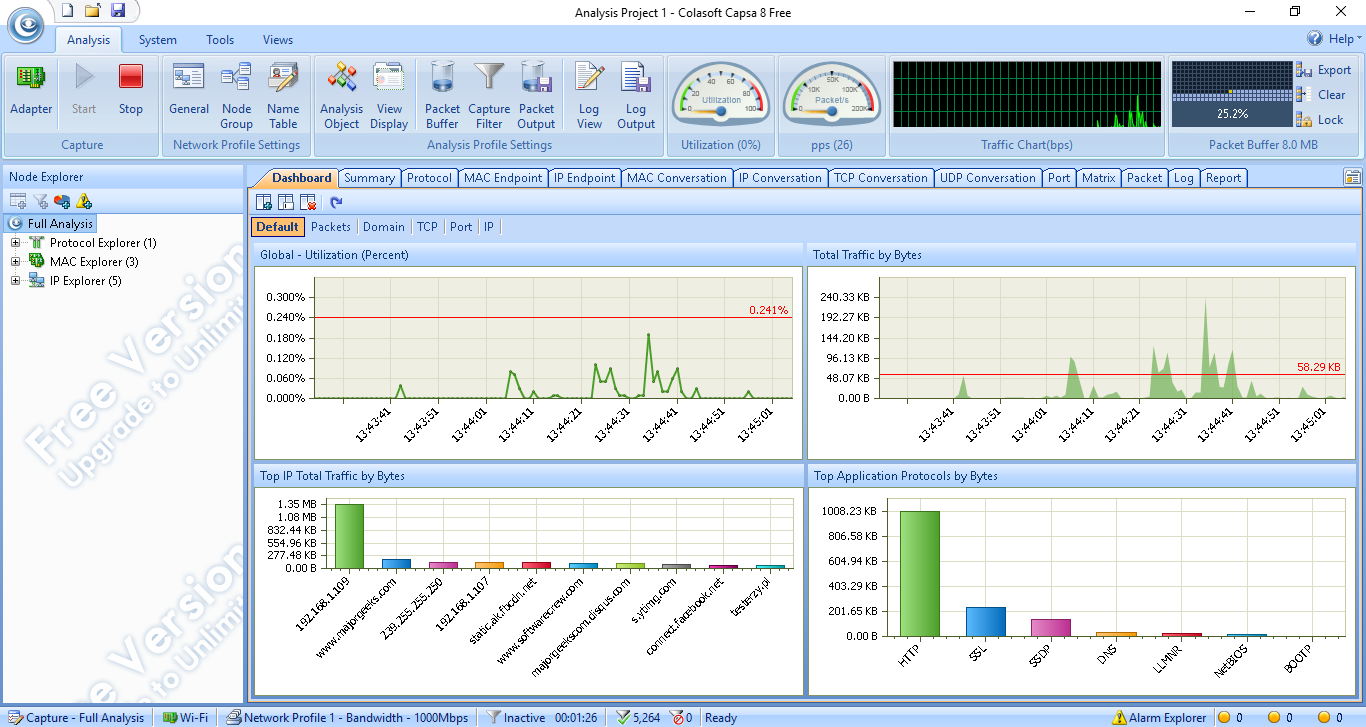
\includegraphics[width=\linewidth]{\commonSecPathPrefix/sec_1/content/colasoft_capsa.png}
    \caption{Окно программы Colasoft Capsa}
    \label{fig:colasoft}
\end{figure}

Основные характеристики программы Colasoft Capsa:
\begin{itemize}
    \item поддержка ОС: все 32-битные и 64-битные версии Windows XP;
    \item минимальные системные требования: 4 Гб оперативной памяти и
    процессор 2,8 ГГц;
    \item хорошо работает со всеми проводными и беспроводными интерфейсами,
    включая Bluetooth, Wi-Fi и Ethernet (совместимый с NDIS 3 или выше).
\end{itemize}

Программа имеет платную версию и бесплатную с урезанным функционалом. На бесплатную 
версию накладываются ограничения по времени сессии работы анализатора, отстутствует
возможность сохранять данные, просматривать информацию в определенных режимах и так далее.


\subsubsection{SolarWinds NetFlow Analyzer}

SolarWinds NetFlow Analyzer является одним из наиболее популярных
программных инструментов для анализа сетевого трафика и мониторинга
пропускной способности, который поддерживает работу с различными
протоколами, включая: NetFlow, J-Flow, sFlow, IPFIX и NetStream. Он дает
возможность сортировать, помечать и отображать данные различными
способами. Это позволяет удобно визуализировать и анализировать сетевой
трафик. Инструмент отлично подходит для мониторинга сетевого трафика по
типам и периодам времени, а также для определения того, сколько трафика
потребляют различные приложения.


Таким образом, с помощью SolarWinds NetFlow Analyzer можно
изучать и устранять неполадки и спады в функционировании сети, а также
определять пользователей, приложения и устройства, которые используют
больше всего ресурсов сети. Окно программы представлено на рисунке \ref{fig:solarwinds}.

\begin{figure}[h!]
    \centering
    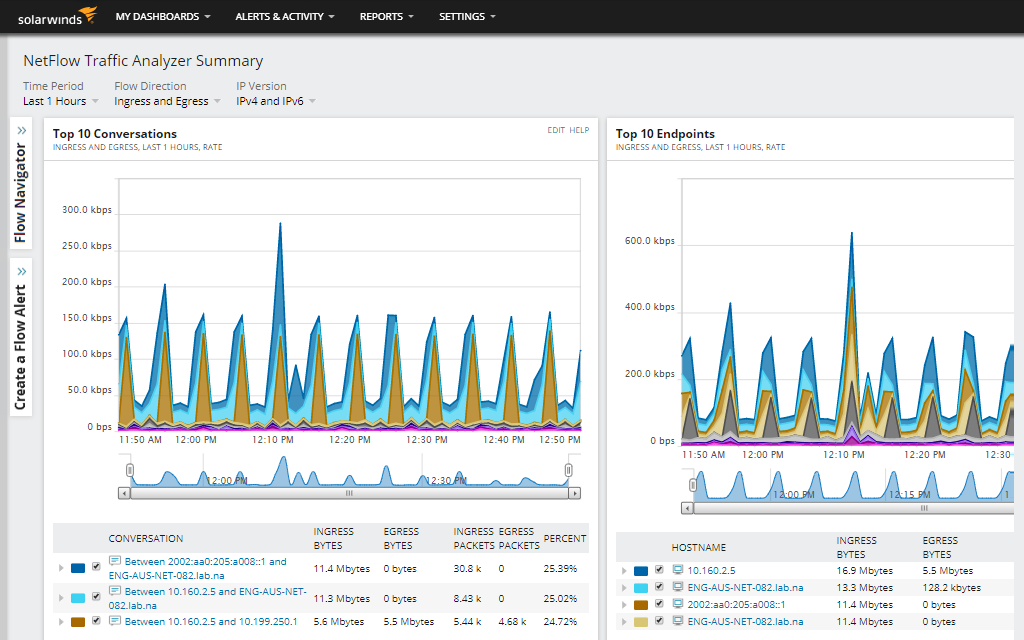
\includegraphics[width=\linewidth]{\commonSecPathPrefix/sec_1/content/solarwinds_netflow.png}
    \caption{Окно программы SolarWinds NetFlow Analyzer}
    \label{fig:solarwinds}
\end{figure}

Основные характеристики программы SolarWinds NetFlow Analyzer:
\begin{itemize}
    \item использование баз данных SQL;
    \item поддержка ОС: Windows 11, 10, 8, 7;
    \item рекомендации скорости процессора, объему оперативной памяти и
    скорости сетевого адаптера варьируются в зависимости от количества
    отслеживаемых сетевых элементов.
\end{itemize}

Продукт является платным, однако любой желающий может воспользоваться пробным 
периодом в 30 дней, по истечении которого все же придется купить платную версию.


\subsubsection{Ntopng}

Ntopng -- это веб-инструмент с открытым исходным кодом для
мониторинга и анализа сетевого трафика на основе данных о потоке и
статистики, извлеченной из наблюдаемого трафика. Через зашифрованный
интерфейс поступают данные о переданных пакетах. Программа анализирует их
и предоставляет различную полезную информацию о функционировании вашей
сети. Окно программы представлен на рисунке \ref{fig:ntopng}.

\begin{figure}[h!]
    \centering
    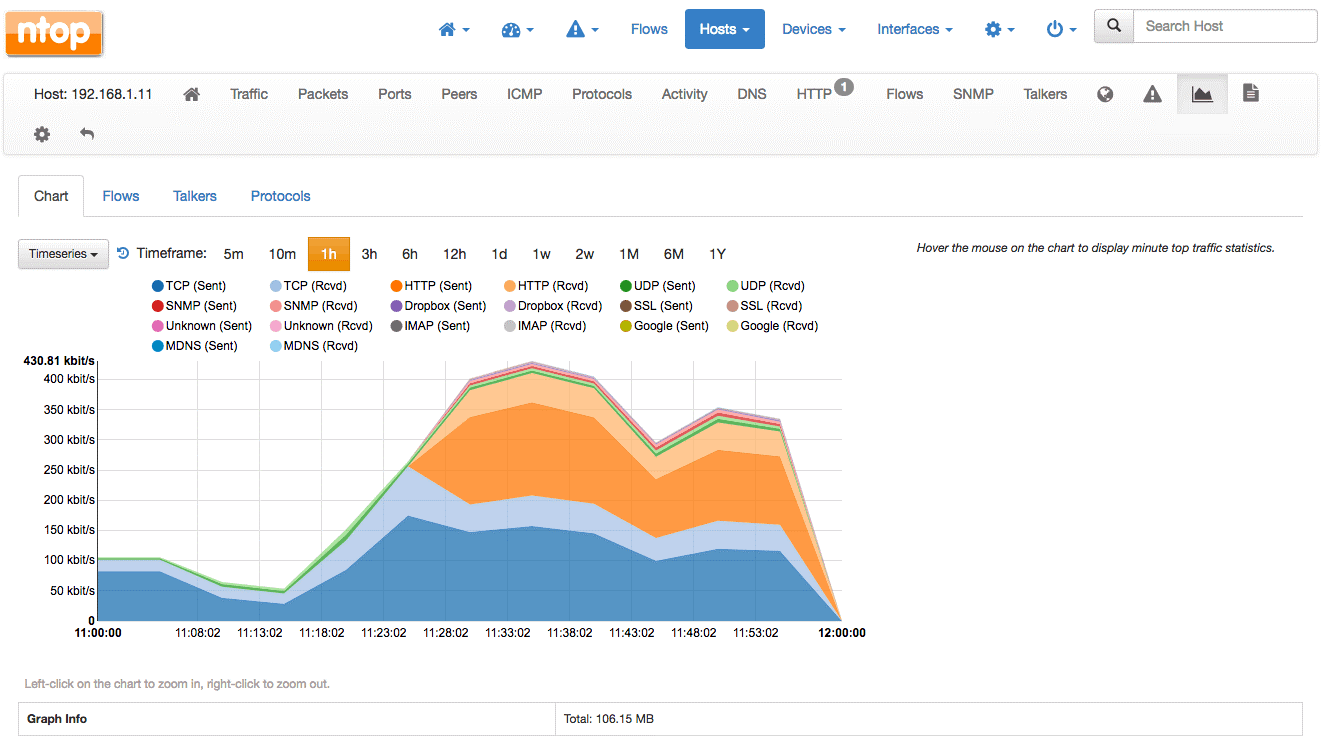
\includegraphics[width=\linewidth]{\commonSecPathPrefix/sec_1/content/ntopng.png}
    \caption{Окно программы Ntopng}
    \label{fig:ntopng}
\end{figure}

С помощью ПО Ntopng вы можете:
\begin{itemize}
    \item сортировать информацию о сетевом трафике по многим параметрам,
    включая IP-адреса, порты, протоколы, пропускную способность и т. д.;
    \item в режиме реального времени отслеживать наиболее активные хосты и
    приложения, требующие больше всего пропускной способности;
    \item отслеживать информацию о переданных байтах, а также количество
    отправленных, полученных и потерянных пакетов;
    \item сохранять на диск историю сетевого трафика для последующего анализа;
    \item отображать задержку и статистику TCP (например, потерю пакетов);
    \item определять географическое местоположение и строить схемы соединения
    хостов на карте местности.
\end{itemize}


Поскольку Ntopng является приложением с открытым исходным кодом, существует
множество возможностей для его расширения. Данные можно экспортировать в
MySQL, ElasticSearch и LogStash, где они могут быть объединены в отчеты,
хранящиеся на сервере Syslog.


Программа Ntopng может подключаться к nProbe, который является
коллектором NetFlow/IPFIX. В этом тандеме роли распределены следующим
образом: nProbe собирает данные о потоках и отправляет эту информацию в
Ntopng, который, в свою очередь, анализирует ее и представляет в удобном для
восприятия виде.


Основные характеристики:
\begin{itemize}
    \item поддержка ОС: Linux, MacOS и Windows х64;
    \item полная поддержка IPv4 и IPv6;
    \item поддержка TLS/HTTPS;
    \item доступно через любой веб-браузер, поддерживающий HTML 5.
\end{itemize}

Общедоступная версия является бесплатной и ее открытый код находится в репозитории 
разработчиков на GitHub. Однако существует также корпоративная и «про» версии с 
расширенным функционалом, предназначенные для использования в коммерческих целях.


